\chapter{Spielvorstellung}
\section{Spielmechanik}
%Was soll passieren
%Was ist Sinn hinter dem Spiel
%Karte zu beginn -> Karte des Spiels am Ende -> Evolution der Entwicklung
Die Idee meiner Gruppe, war es ein Spiel zu entwerfen, welches zusätzlich zu den unterhaltenden Faktor auch noch einen lehrenden Einfluss besitzt. In einer virtuellen Welt spielt der Spieler einen Igel in First-Person. Dazu kann sich der Spieler mit den Controllern auf der Karte, welche in \autoref{fig:map} dargestellt ist, fortbewegen. Im Laufe des Spiels lernt der Anwender wissenswertes über Igel und muss sein Wissen bei den verschiedenen Stationen auf die Probe stellen. Das erfolgreiche Bearbeiten der Stationen ist nötig, da man als Errungenschaft jeweils ein Blatt erhält. Wenn alle Blätter gesammelt wurden, wird das Spiel im Haus der Igelfamilie beendet.

\begin{figure}[H]
	\centering
	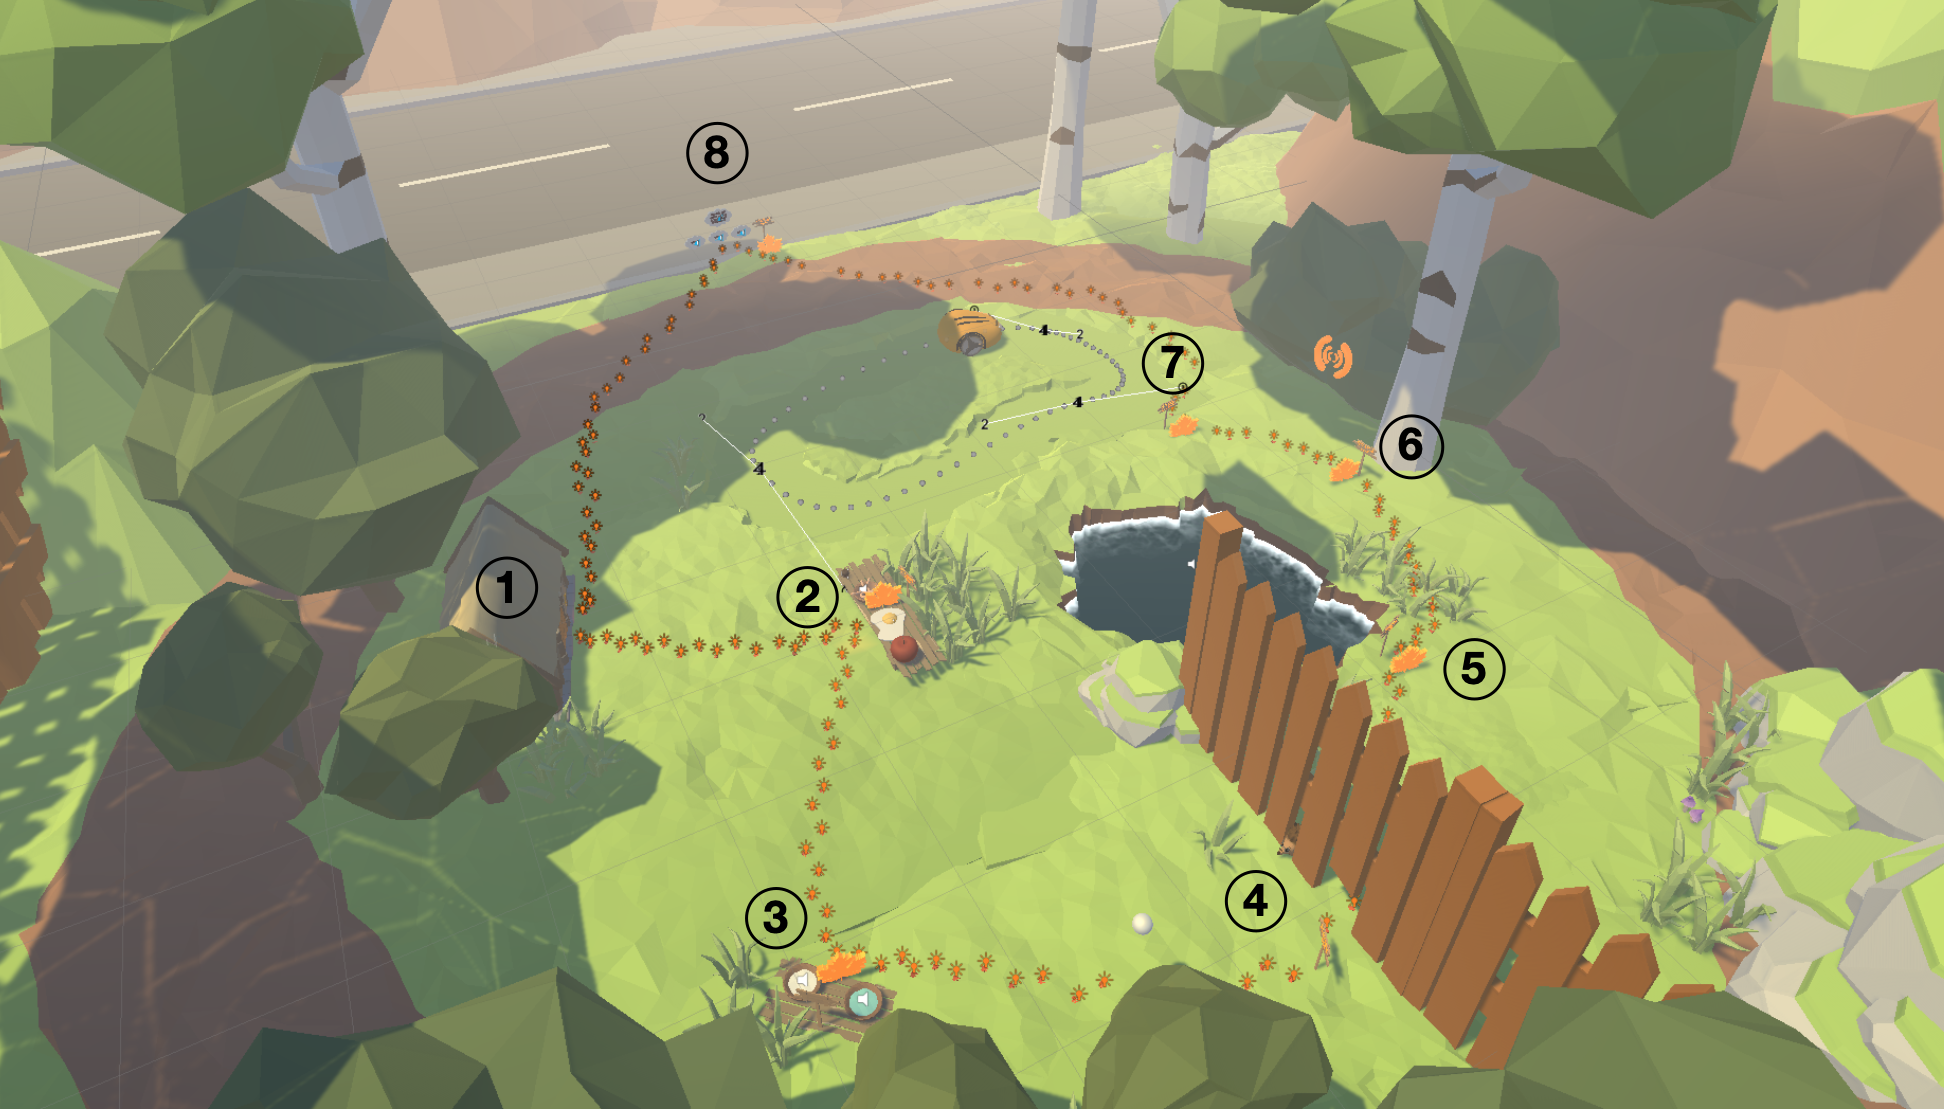
\includegraphics[width=0.675\linewidth]{map.png}
	\caption[Übersicht über die Spielkarte]{Übersicht über die Spielkarte 1: Tutorial, 2: Essen, 3: Trinken, 4: Zaun, 5: Teich, 6: Feind, 7: Rasenmäher, 8: Straße. Quelle: Eigene Aufnahme}
	\label{fig:map}
\end{figure}
 
Zur Steuerung wurde eine Kombination aus Teleportation und Fortbewegung mit den Joysticks der Controller gewählt. Es wurde keine reine physische Fortbewegung implementiert, da die Karte des Spiels sonst auf die jeweilige begehbare reale Umgebung angepasst werden muss. Damit ist das Spiel auch unabhängig der räumlichen Möglichkeiten spielbar.


\section{Immersion}
Ein Spiel wird als immersiv bezeichnet, wenn der Spieler vollständig in die fiktive Welt eintaucht und dabei die Wahrnehmungen der realen Umgebung sinken oder gänzlich verschwinden. Dies wurde in dem Spiel mithilfe der Größe der modellierten Umgebung versucht zu erreichen. Da ein Igel relativ klein ist, wurde die Welt mit seinen Gegenständen dementsprechend größer modelliert. Dieser Sachverhalt ist in \autoref{fig:big_objects} zu sehen. Für ein schöneres Spielgefühl sind zudem noch Audiobestandteile eingefügt, welche für ein besseres Ambiente sorgen. So sind an der Straße die Autos oder bei der Station des Rasenmähers dieser zu hören.

\begin{figure}[H]
	\centering
	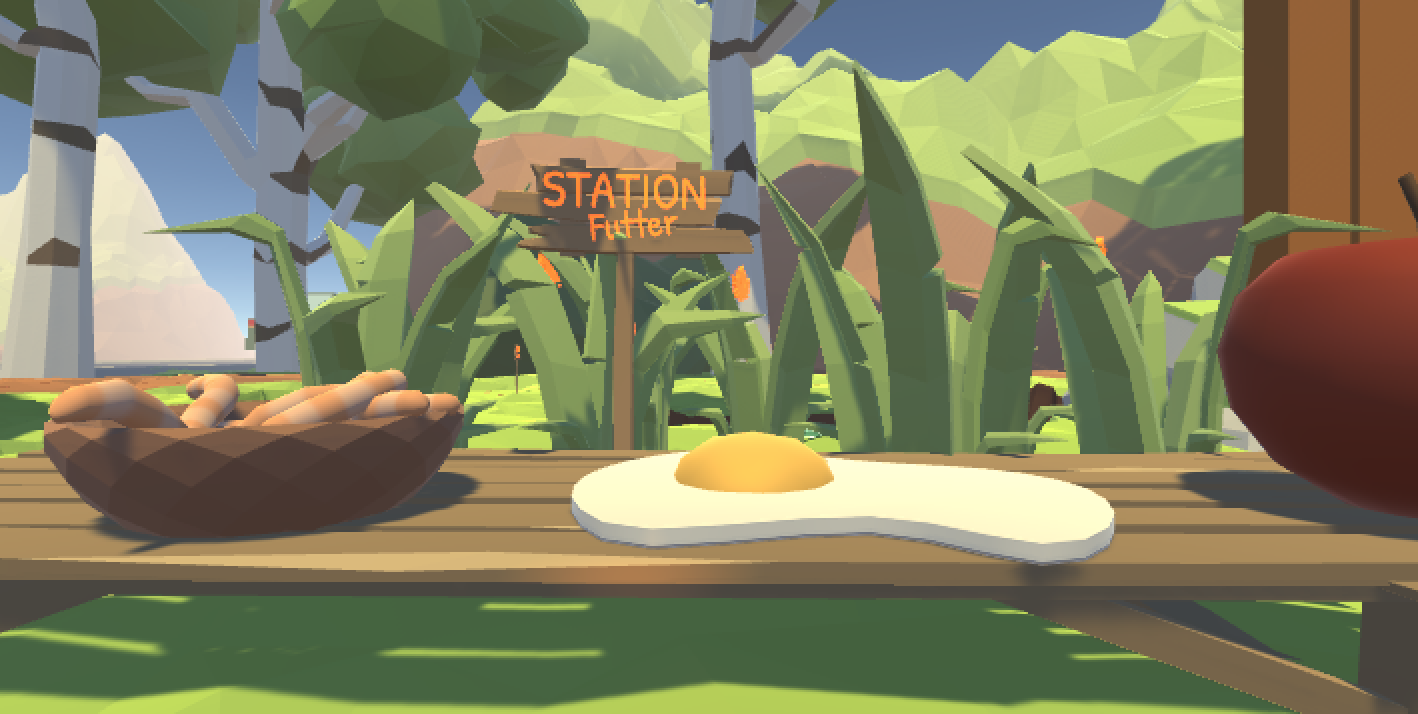
\includegraphics[width=0.55\linewidth]{big_objects.png}
	\caption[Darstellung der Größenunterschiede]{Darstellung der Größenunterschiede. Quelle: Eigene Aufnahme}
	\label{fig:big_objects}
\end{figure}

Es sei aber zu erwähnen, dass durch die Wahl der Fortbewegungsmethode und der Low-Poly Grafik der Effekt der Immersion gemindert wird.
